\documentclass[xcolor=table]{beamer}
\usetheme{Warsaw}
\usepackage[polish]{babel}
\usepackage[utf8]{inputenc}
\usepackage[T1]{fontenc}
\usepackage{amsmath}
\usepackage{graphicx}
\usepackage{tikz} % custom positions
\beamertemplatenavigationsymbolsempty % disable navigatoin bar
\usepackage{changepage} % adjustwidth
\setbeamertemplate{caption}[numbered] % numery w rysunkach
\usepackage{multirow} % spaning columns in tables

\def\tikzoverlay{%
   \tikz[baseline,overlay]\node[every overlay node]
}%




\title[Analiza sentymentu i geolokacja w sieciach społecznych]
{Możliwości powiązania 
\\ danych geolokacyjnych i analizy sentymentu \\
w analizie zachowań użytkowników \\ 
w wybranych portalach społecznościowych}
\author{Dariusz Mydlarz}

\institute[AGH Kraków]{
Promotor: dr inż. Anna Zygmunt
\\ \vspace{0.3cm}
Akademia Górniczo-Hutnicza im. Stanisława Staszica w Krakowie\\
Wydział Informatyki, Elektroniki i Telekomunikacji -- Katedra
Informatyki}

\date{Kraków, 10 grudnia 2014 roku}

\defbeamertemplate*{footline}{shadow theme}
{%
  \leavevmode%
  \hbox{\begin{beamercolorbox}[wd=.5\paperwidth,ht=2.5ex,dp=1.125ex,leftskip=.1cm plus1fil,rightskip=.1cm]{author in head/foot}%
    \usebeamerfont{title in head/foot}\insertshorttitle%
  \end{beamercolorbox}%
  \begin{beamercolorbox}[wd=.5\paperwidth,ht=2.5ex,dp=1.125ex,leftskip=.1cm,rightskip=.1cm plus1fil]{title in head/foot}%
    \usebeamerfont{author in
    head/foot}\insertshortauthor
    \hfill
    \insertframenumber/\inserttotalframenumber \end{beamercolorbox}}%
  \vskip0pt% 
}


% ==================================================================================
\begin {document}
% ==================================================================================
{
\setbeamertemplate{headline}{}
\setbeamertemplate{footline}{}
\begin{frame}
\maketitle
\end{frame}
}


% ==================================================================================
\begin{frame}{Agenda}
\tableofcontents
\end{frame}

% ==================================================================================
\section{Motywacja i cele}
% ==================================================================================
\begin{frame}{Motywacja i cele}
Cel -- zbadanie możliwości połączenia trzech dziedzin:
\begin{itemize}
\item analizy sieci społecznościowych
\item analizy sentymentu
\item geolokacji
\end{itemize}
\vspace{0.5cm}
Motywacje:
\begin{itemize}
\item dziedziny nie łączone wcześniej  
\item ogromna popularność serwisów społecznościowych
\item wykorzystanie szerokiej wiedzy zdobytej na studiach
\end{itemize}
\end{frame}

% ==================================================================================
\section{Sposób realizacji i przebieg prac}
% ==================================================================================
\begin{frame}{Sposób realizacji i przebieg prac}
\begin{enumerate}
  \item zbieranie danych z Twittera
  
  \item wybór i budowa narzędzi do ekstrakcji wiedzy
%  \begin{itemize}
%	\item klasyfikator sentymentu
%  \end{itemize}
  
  \item odkrywanie wiedzy
%  \begin{itemize}
%    \item obliczenie sentymentu wpisów
%	\item identyfikacja zwolenników i przeciwników
%	\item zastosowanie geolokacji
%	\item odkrywanie zachowań użytkowników 
%  \end{itemize}
  
\end{enumerate}

\begin{figure}[ht!]
\centering
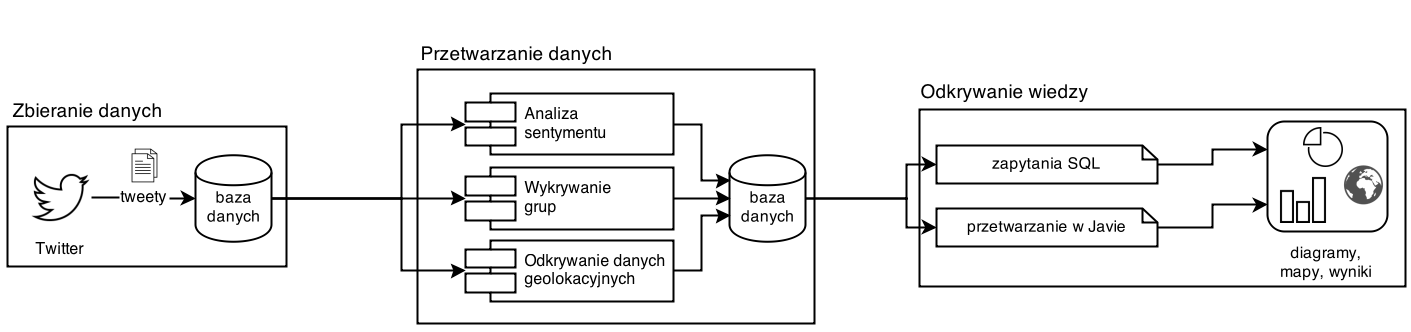
\includegraphics[width=11cm]{img/gruby-model.png}
\caption{Kolejne etapy realizacji systemu}
\end{figure}

\end{frame}

% ==================================================================================
\section{Uzyskane rezultaty}
% ==================================================================================
\begin{frame}{Zebrane dane}
\begin{itemize}
  \item 7 mln tweetów  
  \item 49\% pozytywnych, 47\% negatywnych
\end{itemize}

\begin{figure}[ht!]
\centering
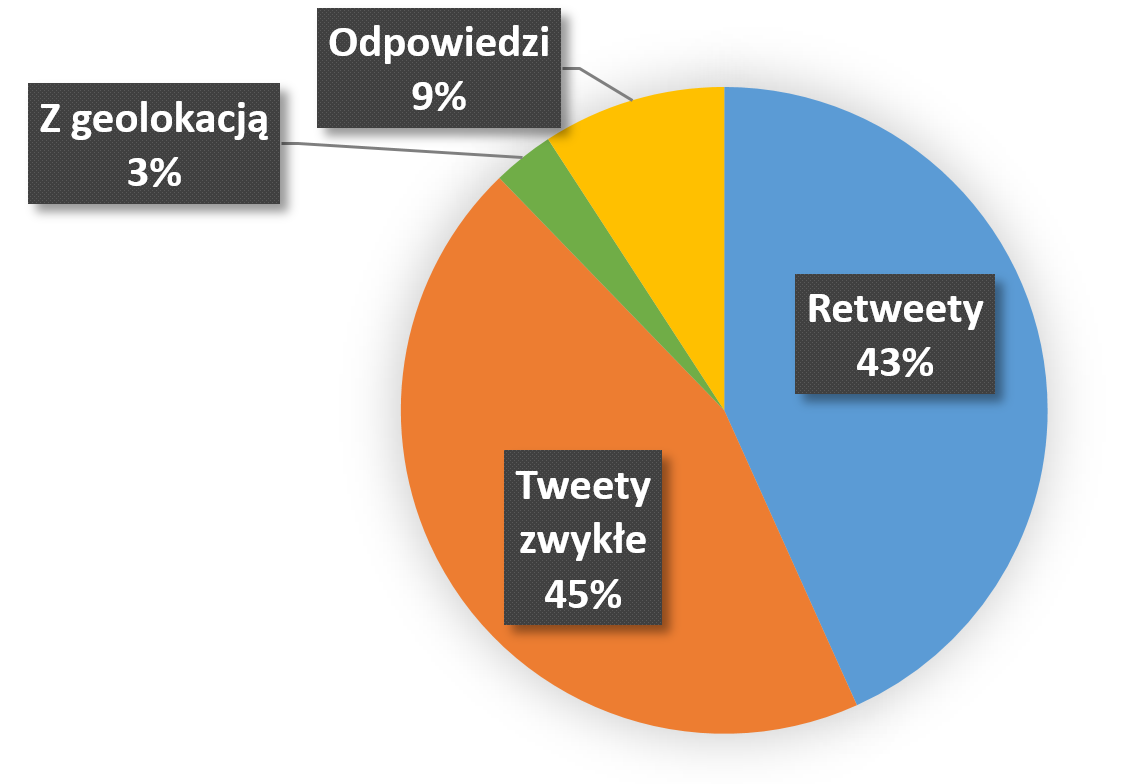
\includegraphics[width=6cm]{img/rozklad-wpisow2.png}
\caption{Struktura zebranych wpisów}
\end{figure}
\end{frame}

% ==================================================================================
\begin{frame}{Aktywność użytkowników i rozkład sentymentu}

\begin{figure}[ht!]
\centering
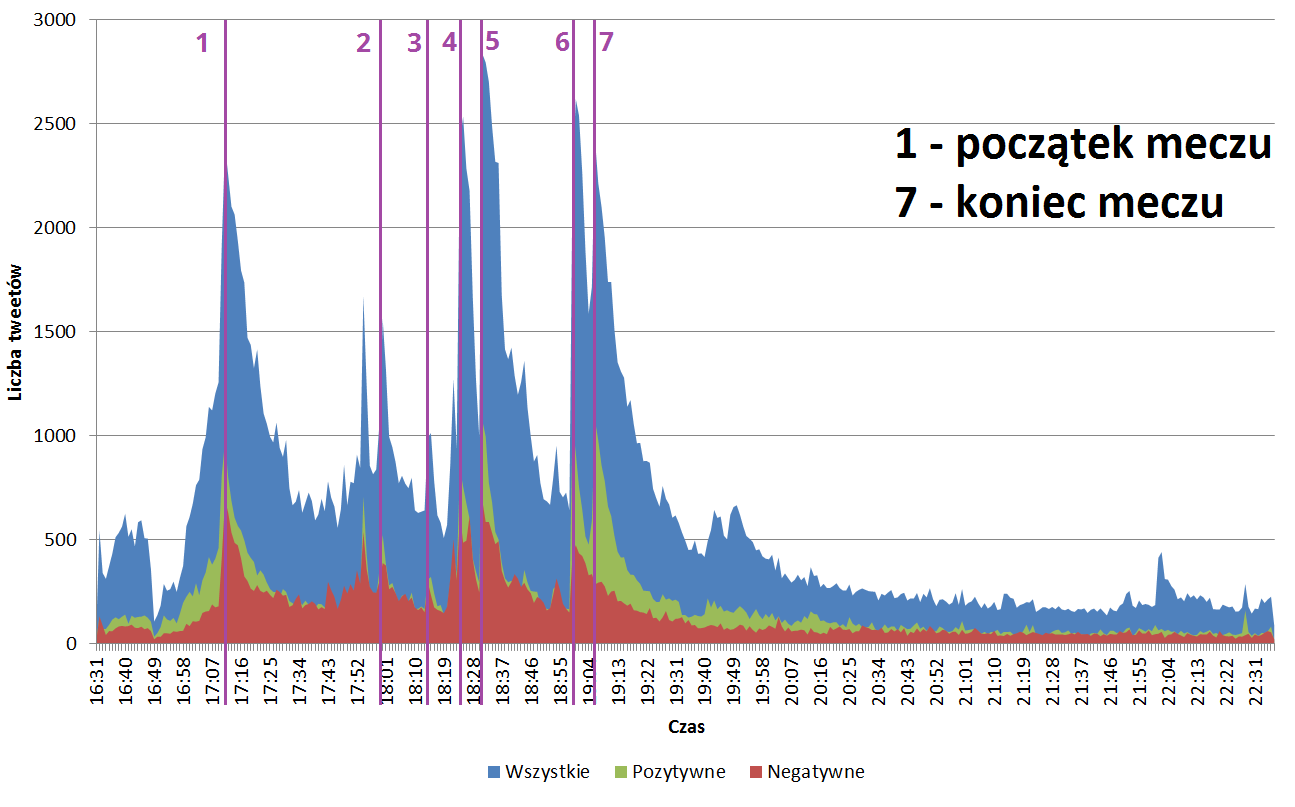
\includegraphics[width=10cm]{img/tweety-w-meczu-nums2.png}
\caption{Zmiana liczby wpisów w czasie}
\end{figure}
 
\end{frame} 

% ==================================================================================
\begin{frame}{Interakcja między użytkownikami}

%\begin{adjustwidth}{-5cm}{-5cm}
%\begin{table}
%\begin{tabular}{rl}
%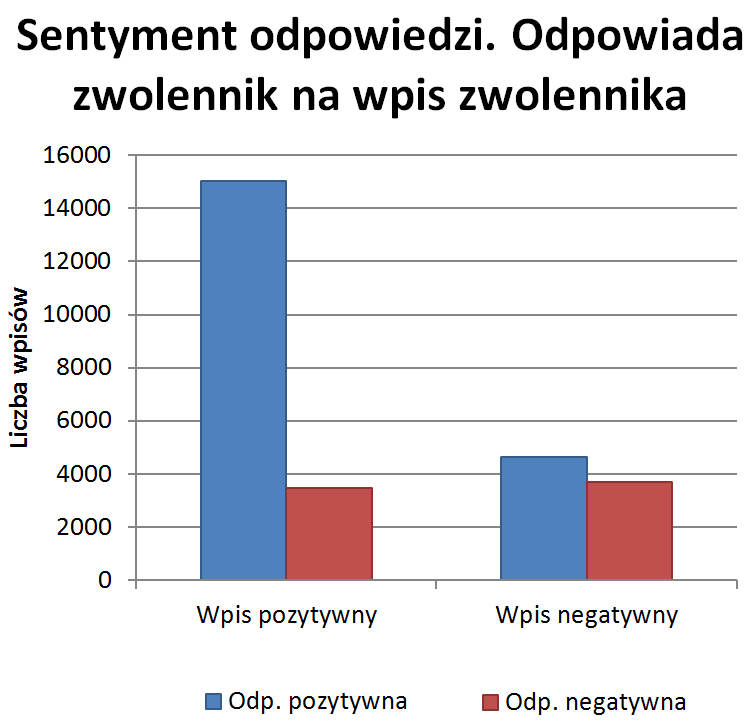
\includegraphics[width=0.50\textwidth]{img/reply-sentiment-zwolennik-zwolennik.PNG}
%&
%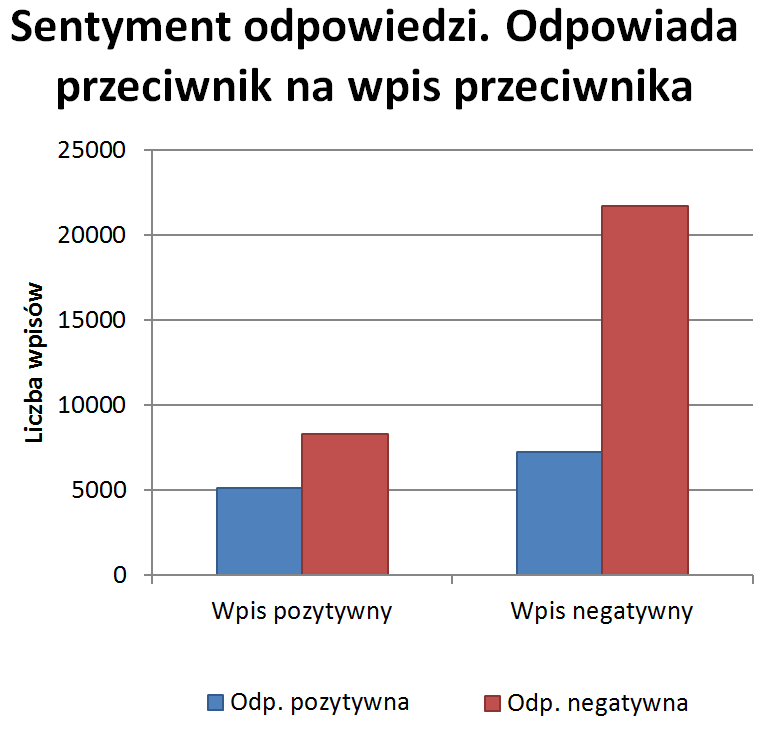
\includegraphics[width=0.50\textwidth]{img/reply-sentiment-przeciwnik-przeciwnik.PNG}
%\end{tabular}
%\end{table}
%\end{adjustwidth}

Sentyment wiadomości między zwolennikami i przeciwnikami klubu

\begin{table}[h]
\begin{tabular}{l|c|r|}
\cline{2-3}
& \multicolumn{2}{c|}{Wiadomości między zwolennikami klubu}          
\\ \cline{2-3} &  
\multicolumn{1}{p{30mm}|}{Wpis pozytywny} &
\multicolumn{1}{p{30mm}|}{Wpis negatywny} \\ \hline

\multicolumn{1}{|c|}{Odp. pozytywna} &
\multicolumn{1}{r|}{\cellcolor[HTML]{34CDF9}15027} & 4661 \\ \hline 
\multicolumn{1}{|c|}{Odp. negatywna} & \multicolumn{1}{r|}{3495} & 3701                                   
\\ \hline
\end{tabular}
\end{table}

\begin{table}[h]
\begin{tabular}{l|c|r|}
\cline{2-3}
& \multicolumn{2}{c|}{Wiadomości między przeciwnikami klubu}          
\\ \cline{2-3} &

\multicolumn{1}{p{30mm}|}{Wpis pozytywny} &
\multicolumn{1}{p{30mm}|}{Wpis negatywny} \\ \hline

\multicolumn{1}{|c|}{Odp. pozytywna} & \multicolumn{1}{r|}{5154} & 7238              
\\ \hline 
\multicolumn{1}{|c|}{Odp. negatywna} & \multicolumn{1}{r|}{8306} &
{\cellcolor[HTML]{34CDF9}21687} \\ \hline
\end{tabular}
\end{table}

\end{frame}

% ==================================================================================
%\begin{frame}{Struktura grup między meczami}
%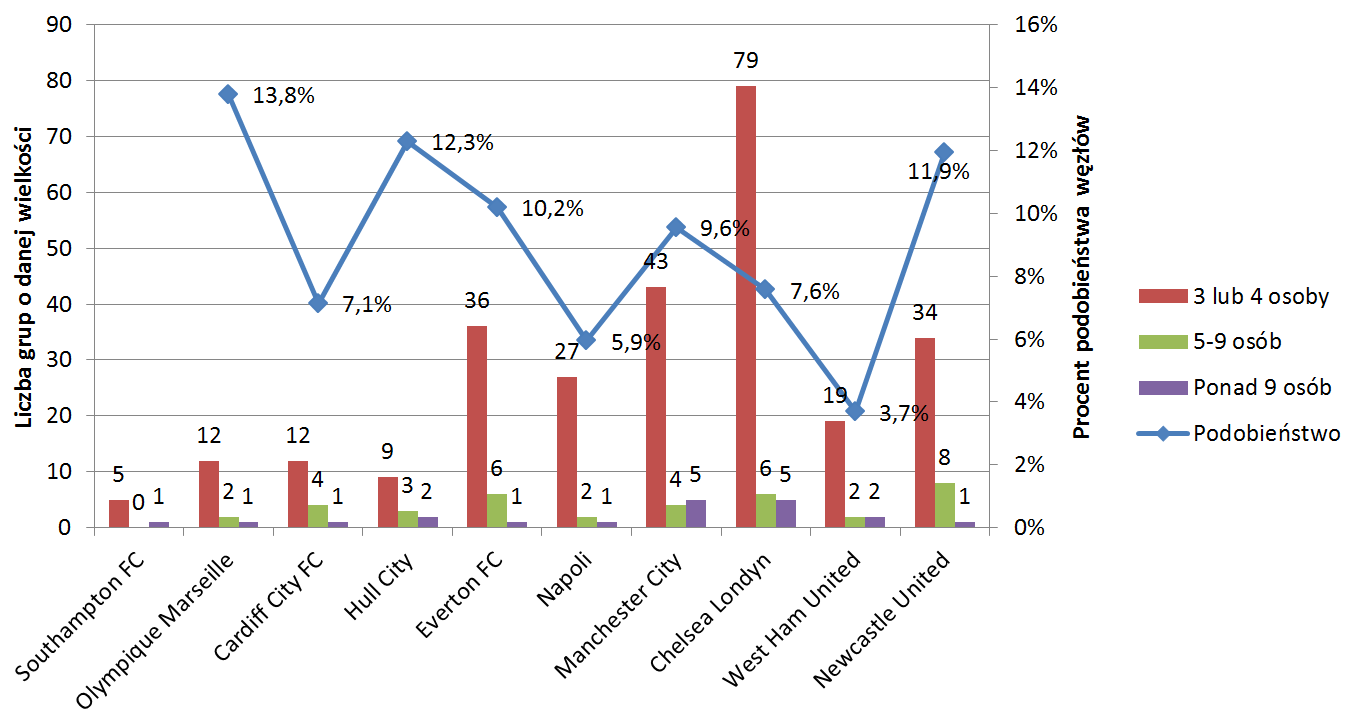
\includegraphics[width=1\textwidth]{img/grupy-arsenal-nums.png}
%\end{frame}

% ==================================================================================
\begin{frame}{Aktywność kibiców, a odległość od stadionu}

Odległość kibiców od stadionu a miejsce rozgrywania spotkania

\begin{columns}[C] % align columns
\begin{column}{.48\textwidth}

\begin{figure}[ht!]
\centering
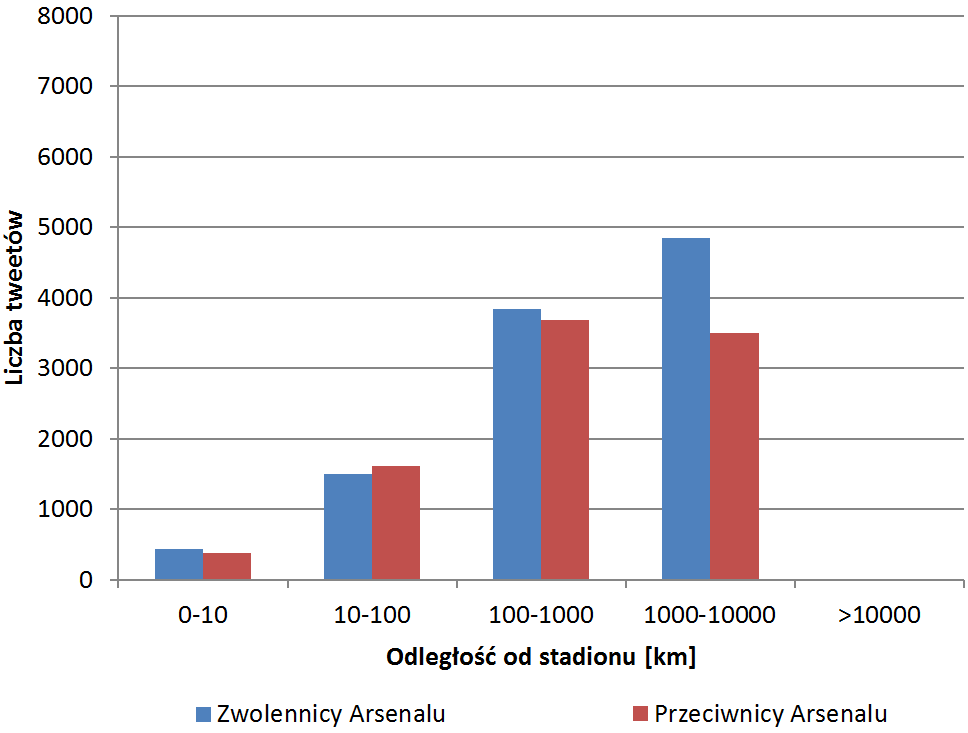
\includegraphics[width=\linewidth]{img/odleglosc-od-stadionu-home.png}
\caption{Mecze u siebie}
\end{figure}

\end{column}%
\hfill%
\begin{column}{.48\textwidth}


\begin{figure}[ht!] 
\centering
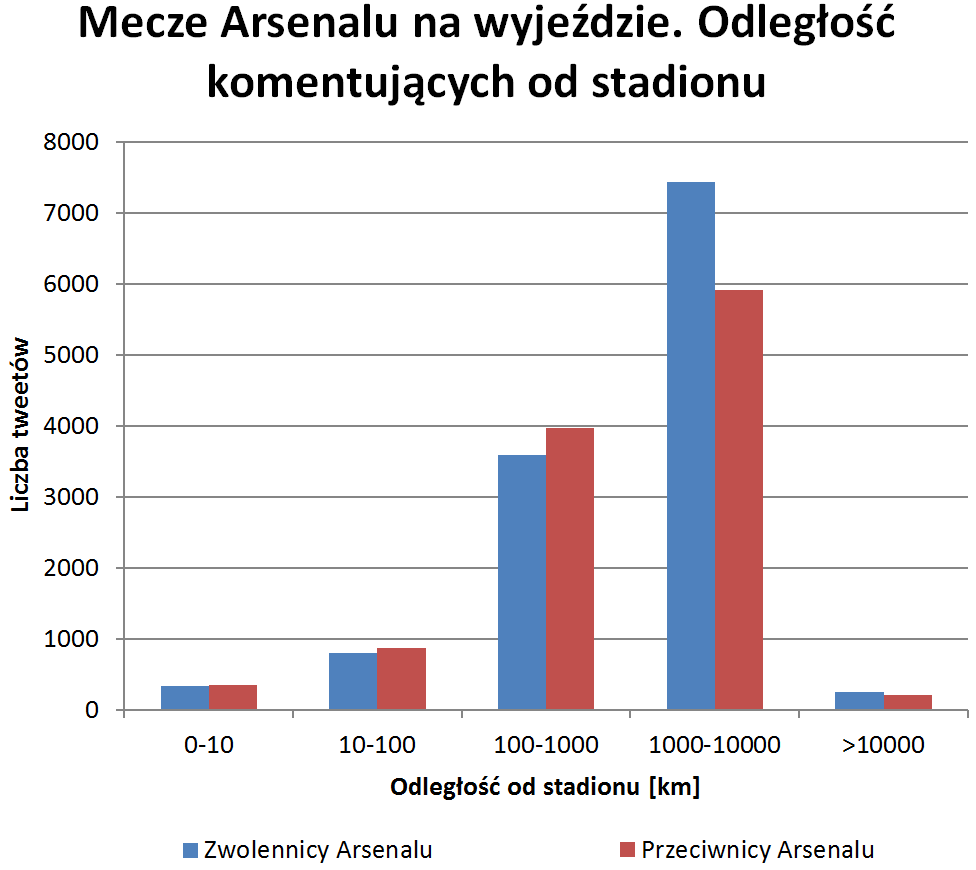
\includegraphics[width=\linewidth]{img/odleglosc-od-stadionu-away.png}
\caption{Mecze na wyjeździe}
\end{figure}

\end{column}%
\end{columns}

\end{frame}

% ==================================================================================
\begin{frame}{Inne eksperymenty}
\begin{enumerate}
  \item struktura grup między meczami
  \begin{itemize}
    \item zauważalna stała grupa kibiców
    \item im bardziej popularne mecze, tym mniejsze podobieństwo użytkowników
    w nich uczestniczących 
  \end{itemize}
  \item zmiana sentymentu w meczach
  \begin{itemize}
    \item gdy drużyna wygrywa -- wydźwięk bardziej pozytywny, gdy przegrywa --
    bardziej negatywny
  \end{itemize}
  \item struktura komunikacji
  \begin{itemize}
    \item przecwinicy najczęściej odpowiadają sobie nazwajem
    \item zwolennicy najczęściej podają swoje wpisy dalej (retweetują)
  \end{itemize}
  \item częstość komunikacji a fizyczna odległość między kibicami
  \begin{itemize}
    \item im kibice fizycznie bliżej siebie, tym częściej się ze sobą komunikują
  \end{itemize} 
   
\end{enumerate}
\end{frame}
% ==================================================================================
\begin{frame}{Podsumowanie eksperymentów}
\begin{itemize}
  \item użytkownicy sieci społecznościowych zachowują się w Internecie w taki
  sam sposób jak w życiu codziennym
  \item najnowsze technologie komputerowe pozwalają na badanie dużych
  społeczności w sposób transparentny
  \item badanie sieci społecznych można zautomatyzować i zastosować również do
  innych dziedzin 
\end{itemize}
\end{frame}


% ==================================================================================
\appendix
% ==================================================================================
\begin{frame}{Podsumowanie pracy}
Osiągnięte cele:
\begin{itemize}
\item połączono geolokację, sentyment i sieci społeczne
\item zbudowano narzędzie do przetwarzania dużej ilości danych z~Twittera pod
kątem analizy sieci społecznych
\item odkryto ciekawe zależności w badanej społeczności
\end{itemize}
\vspace{0.5cm}
Możliwe kierunki rozwoju:
\begin{itemize}
\item rozbudowanie narzędzia do analizy sentymentu
\item odkrywanie tematów rozmów
\item bliższe przyjrzenie się grupom
\end{itemize} 
 
\end{frame} 
 
\end{document}
